\chapter{System maintenance}

The photomultiplier tubes are analog devices, with characteristics
that are influenced by the age and the history of the device. To
produce correct images, some corrections are applied (section
\pref{sec:corrections}). The most important are the linearity
correction and the energy correction. In most cameras, there is an
additional correction, called the uniformity correction, taking care
of remaining second order deviations. It is important to keep on eye
on the camera performance and tune it every now and then. Failure to
do so will lead to gradual deterioration of image quality.

When a camera is first installed, the client tests it extensively to
verify that the system meets all required specifications (the
acceptance test). The National Electrical Manufacturers Association
(NEMA, ``national'' is the USA here) has defined standard protocols to
measure the specifications. The standards are widely accepted, such
that specifications from different vendors can be compared, and that
discussions between customers and companies about acceptance test
procedures can be avoided. You can find information on {\em
http://www.nema.org}.

This chapter gives an overview of tests which provide valuable information on
camera performance. Many of these tests can be done quantitatively: they
provide a number. {\em It is very useful to store the numbers and plot them as
a function of time:} this helps detecting problems early, since gradual
deterioration of performance is detected on the curve even before the
performance deteriorates beyond the specifications.

Quality control can be tedious sometimes, and it is not productive on
the short term: it costs time, and if you find an error, it also costs
money. Most of the time, the camera is working well, so if you assume
that the camera is working fine, you are probably right and you save
time. This is why a quality control program needs continuous
monitoring: if you don't insist on quality control measurements, the
QC-program will silently die, and image quality will slowly
deteriorate.

\section{Gamma camera}
%%%%%%%%%%%%%%%%%%%%%%
For gamma camera quality control and acceptance testing, the {\em Nederlandse
Vereniging voor Nucleaire Geneeskunde} has published a very useful book
\cite{Aanbevelingen}. It provides detailed recipes for applying the
measurement and processing procedures, but does not attempt to explain it, the
reader is supposed to be familiar with nuclear medicine. These explanations
can be found in ``het Leerboek Nucleaire Geneeskunde'' \cite{Leerboek}.


\begin{figure}[tb]
\centering
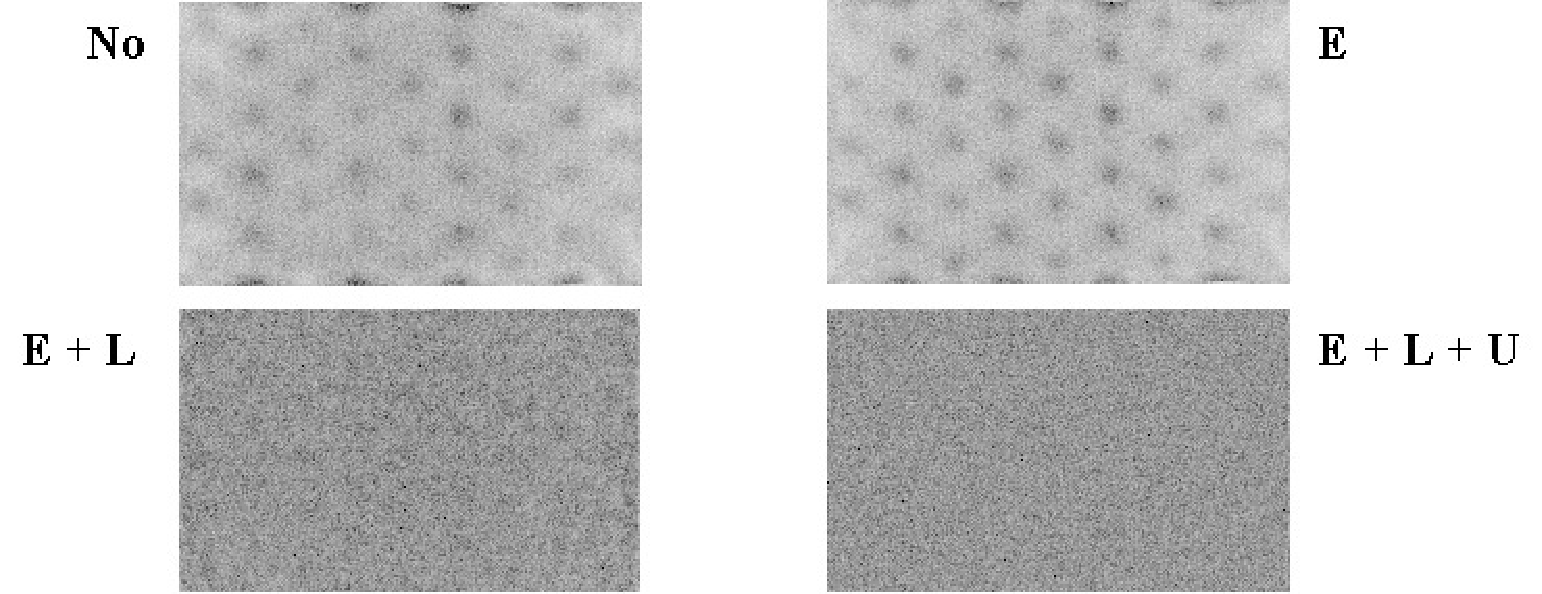
\includegraphics[width=\figbig]{figs/fig_en_lin_unif.pdf}
\caption{\label{fig:en_lin_unif} \emph{Image of a uniform phantom. E = energy
correction, L = linearity correction, U = uniformity correction.}}
\end{figure}
%
Figure \ref{fig:en_lin_unif} shows the influence of the corrections on the
image of a uniform phantom. Without any correction, the photomultipliers are
clearly visible as spots of increased intensity. After energy correction this
is still the case, but the response of the PMTs is more uniform. When in
addition linearity correction is applied, the image is uniform, except for
Poisson noise. Uniformity correction produces a marginal improvement which is
hardly visible.

For most properties, specifications are supplied for the UFOV (usable field of
view) and the CFOV (central field of view). The reason is that performance
near the edges is always slightly inferior to performance in the center. Near
the edges, the scintillation point is not nicely symmetrically surrounded by
(nearly) identical PMTs. As a result, deviations are larger and much stronger
corrections are needed, unavoidably leading to some degradation. The width of
the CFOV is 75\% of the UFOV width, both in $x$ and $y$ direction. 

Quality control typically involves
\begin{itemize}
  \item daily visual verification of image uniformity,
  \item weekly quantitative uniformity testing,
  \item monthly spatial resolution testing
  \item extensive testing every year or after major interventions.
\end{itemize}
The scheme can be adapted according to the strengths and weaknesses of the
systems.


\subsection{Planar imaging}
%==========================
\subsubsection{Uniformity}
%--------------
Uniformity is evaluated by acquiring a uniform image. As a phantom, either
a point source at large distance is measured without collimator, or a
uniform sheet source is put on the collimator. It is recommended to do a quick
uniformity test in the morning, to make sure that the camera seems to work
fine before you start imaging the first patient. Figure \ref{fig:qc_pmt} shows
a sheet source image on a camera with a defect photomultiplier. Of course, you
do not want to discover such a defect with a patient image.
%
\begin{figure}[tb]
\centering
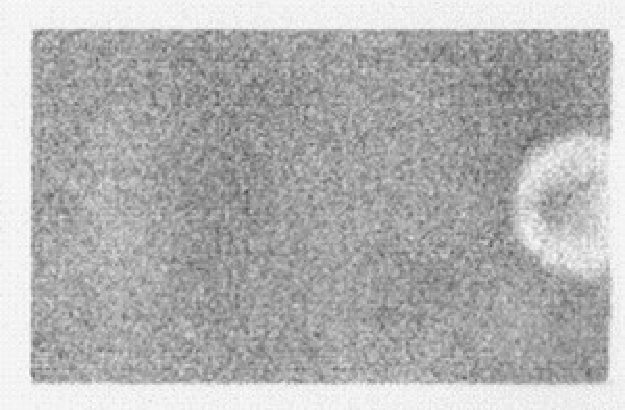
\includegraphics[width=\figone]{figs/fig_qc_pmt.pdf}
\caption{\label{fig:qc_pmt} \emph{Uniform image acquired on a gamma camera
with a dead photomultiplier.}}
\end{figure}

For quantitative analysis, the influence of Poisson noise must be minimized by
acquiring a large amount of counts (typically 10000) per pixel. Acquisition
time will be in the order of an hour. Two parameters are computed from an
image reduced to 64 $\times$ 64 pixels:
\begin{eqnarray}
 \mbox{Integral uniformity} & = & \frac{max - min}{max + min} \times 100 \%
      \label{eq:int_unif}\\
 \mbox{Differential uniformity} & = & \max_{i=1..N} \left( \mbox{regional
 uniformity $i$}, \right)
\end{eqnarray}
where the regional uniformity is computed by applying (\ref{eq:int_unif}) to a
small line interval containing only 5 pixels, and this for all possible
vertical and horizontal line intervals. The differential uniformity is always
a bit smaller than the integral uniformity, and insensitive to gradual changes
in image intensity.

In an image of 64 $\times$ 64 with 10000 counts per pixel, the integral
uniformity due to Poisson noise only is about 4\%, typical specifications are
a bit larger, e.g. 4.5\%.

To acquire a uniformity correction matrix, typically 45000 counts per pixel
are acquired. {\em It is important that the camera is in good shape when a
uniformity correction matrix is produced}. Figure \ref{fig:qc_linproblem}
shows a flood source image acquired on a camera with a linearity correction
problem. The linearity problem causes deformations in the image: counts are
mispositioned. In a uniform image this leads to non-uniformities, in a line
source image to deformations of the line. If we now acquire a uniformity
correction matrix, the corrected flood image will of course be uniform.
However, the line source image will still be deformed, and in addition the
intensities of the deformed line will become worse if we apply the correction
matrix! If uniformity is poor after linearity and energy correction, do not
fix it with uniformity correction. Instead, try to figure out what happens or
call the service people from the company.

The uniformity test is sensitive to most of the things that can go wrong with
a camera, but not all. One undetected problem is deterioration of the pixel
size, which stretches or shrinks the image in $x$ or $y$ direction.

\begin{figure}[tb]
\centering
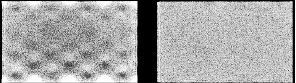
\includegraphics[width=\figbig]{figs/fig_qc_linproblem.pdf}
\caption{\label{fig:qc_linproblem} \emph{Flood source (= uniform sheet source)
image acquired on a dual head gamma camera, with a linearity correction
problem in head 1 (left)}}
\end{figure}

\subsubsection{Pixel size}
%--------------
The $x$ and $y$ coordinates are computed according to equation
(\pref{eq:gammaposition}), so they are affected by the PMT characteristics, the
amplification of the analogue signals prior to A/D conversion and possibly by
the energy of the incoming photon, since that affects the PMT outputs.

Measuring the pixel size is simple: put two point sources at a known distance,
acquire an image and measure the distance in the image. Sub-pixel accuracy is
obtained by computing the mass center of the point source response. The
precision will be better for larger distances. The pixel size must be measured
in $x$ {\em and} in $y$ direction, since usually each direction has its own
amplifiers.

Figure \ref{fig:qc_gain} shows an example where the $y$-amplifier gain
is wrong for one of the heads of a dual head camera (the $x$-gain is
better but not perfect either). The error is found from this dot
phantom measurement by superimposing both images. Since the images are
recorded simultaneously, the dots from one head should fit those from
the other. Because of the invalid $y$-pixel size in one of the heads
there is position dependent axial blurring (i.e. along the y-axis),
which is worse for larger $y$ values.

It is useful to verify if the pixel size is independent of the energy. This
can be done with a $^{67}$Ga point source, which emits photons of 93, 184 and
296 keV. Using three appropriate energy windows, three point source images are
obtained. The points should coincide when the images are superimposed. Repeat
the measurement at a few different positions (or use multiple point sources).

\begin{figure}[tb]
\centering
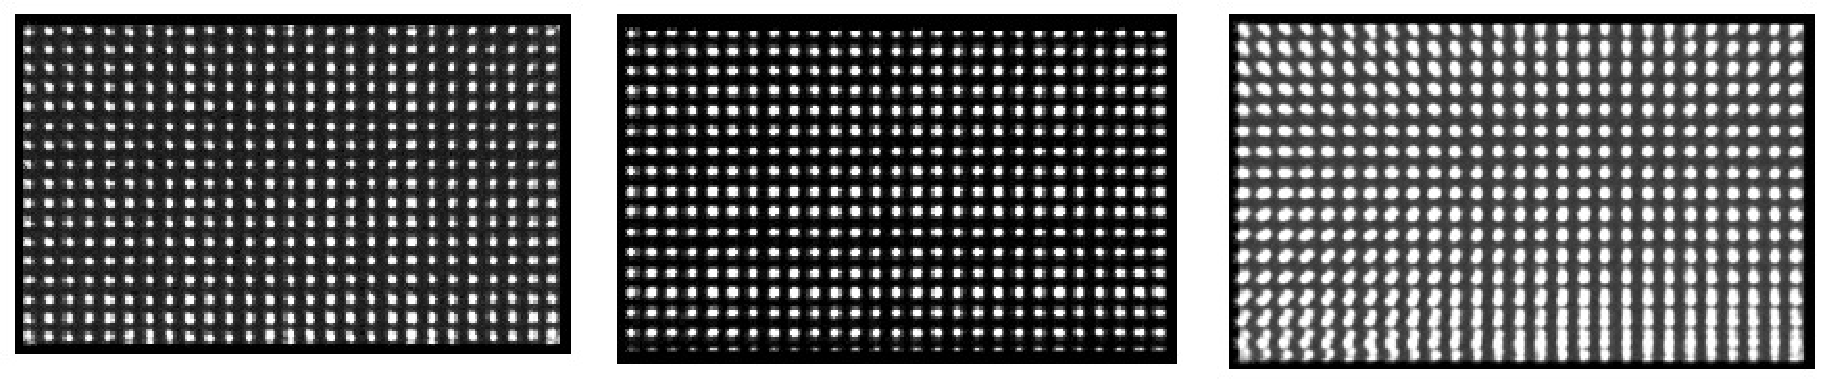
\includegraphics[width=\figbig]{figs/fig_qc_gain.pdf}
\caption{\label{fig:qc_gain} \emph{Images of a dot phantom acquired on a dual
head camera with a gain problem. Left: image acquired on head 1. Center: image
simultaneously acquired on head 2. Right: superimposed images: head1 + mirror
image of head2. The superimposed image is blurred because the heads have a
different pixel size.}}
\end{figure}


\subsubsection{Spatial resolution}
%--------------
In theory, one could measure the FWHM of the PSF directly from a point source
measurement. However, a point source affects only a few pixels, so the FWHM
cannot be derived with good accuracy. Alternatively, one can derive it from
line source measurements. The line spread function is the integral of the
point spread function, since a line consists of many points on a row:
\begin{equation}
  \mbox{LSF}(x) = \int_{-\infty}^{\infty} \mbox{PSF}(x,y) dy.
\end{equation}
Usually, the PSF can be well approximated as a Gaussian curve. The LSF is then
easy to compute:
\begin{equation}
  \mbox{LSF}(x)  =  \int_{-\infty}^{\infty} 
    \frac{1}{2 \pi \sigma^2} e^{- \frac{x^2 + y^2}{2 \sigma^2}} dy
 \;\; = \;\; \frac{1}{\sqrt{2 \pi} \sigma} e^{- \frac{x^2}{2 \sigma^2}}.
\end{equation}
In these equations, we have assumed that the line coincides with the
$y$-axis. So it is reasonable to assume that the FWHM of the LSF is the same
as that of the PSF.  On a single LSF, several independent FWHM measurements
can be done and averaged to improve accuracy. Alternatively, if the line is
positioned nicely in the $x$ or $y$ direction, one can first compute an
average one-dimensional profile by summing image columns or rows and use that
for LSF computations.  Again, measurements for $x$ and $y$ must be made
because the resolution can become anisotropic.

\subsubsection{Energy resolution}
%--------------
Most gamma cameras can display the measured energy spectrum. Because it is not
always clear where the origin of the energy axis is located, it is save to use
two sources with a different energy, and calibrate the axis from the
measurement. E.g. figure \ref{fig:qc_enresol} shows two spectra, one for
\textsuperscript{99m}Tc\ (peak at 140 keV) and the other one for $^{57}$Co (peak at 122
keV). The distance between the two peaks is 18 keV, and can directly be
compared to the FWHM of the two spectra.

The FWHM is usually specified relative to the peak energy. So a FWHM of 10\%
for \textsuperscript{99m}Tc\ means 14 keV.

\begin{figure}[tb]
\centering
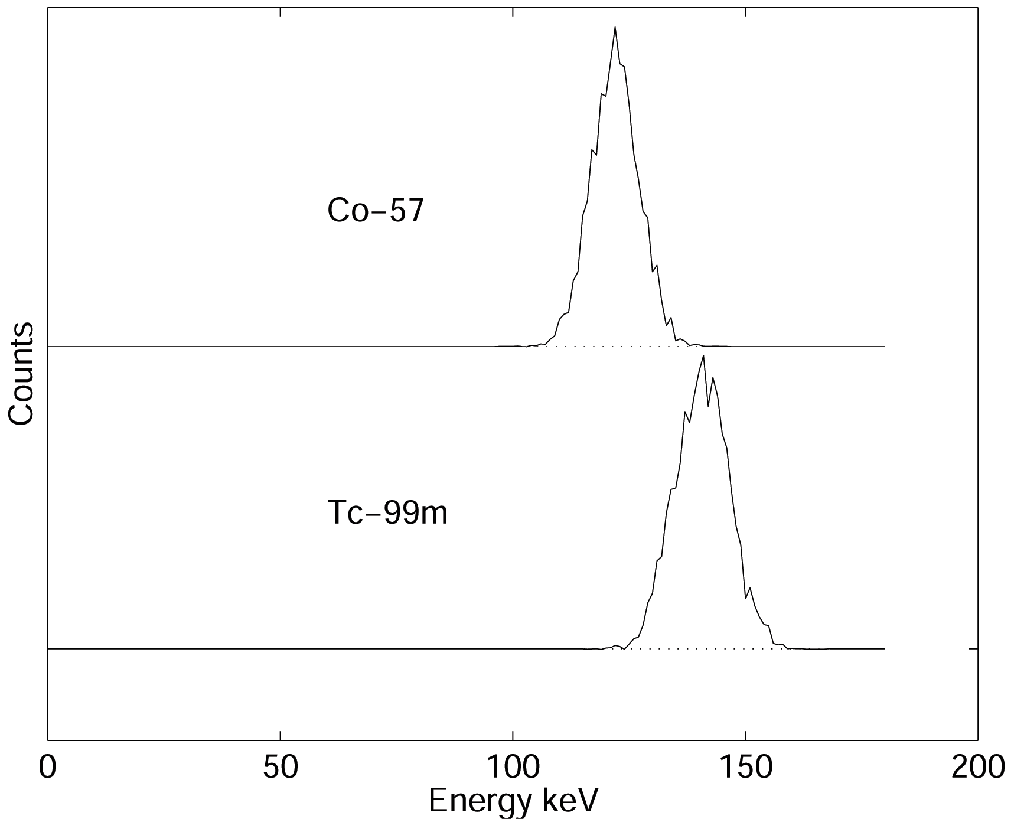
\includegraphics[width=\figone]{figs/fig_qc_enresol.pdf}
\caption{\label{fig:qc_enresol} \emph{(Simulated) energy spectra of Cobalt
($^{57}$Co, 122 keV) and technetium (\textsuperscript{99m}Tc, 140 keV).}}
\end{figure}

\subsubsection{Linearity}
%--------------
The linearity is measured with a line source phantom as shown in
figure \ref{fig:qc_linearity}. This can be obtained in several
ways. One is to use a lead sheet with long slids of 1 mm width,
positioned at regular distances (e.g. 3 cm distance between the
slids). Remove the collimator (to avoid interference between the slids
and the collimator septa, possibly resulting in beautiful but useless
Moir\'{e} patterns), put the lead sheet on the camera (very carefully,
the fragile crystal is easily damaged and very expensive!) and
irradiate with a uniform phantom or point source at large distance.

NEMA states that {\em integral linearity} is defined as the maximum distance
between the measured line and the true line. The true line is obtained by
fitting the known true lines configuration to the image.

The NEMA definition for the {\em differential linearity} may seem a bit
strange. The procedure prescribes to compute several image profiles
perpendicular to the lines. From each profile, the distances between
consecutive lines is measured, and the standard deviation on these distances is
computed. The maximum standard deviation is the {\em differential linearity}.
This procedure is simple, but not 100\% reproducible.

With current computers, it is not difficult to implement a better and more
reproducible procedure. However, a good standard must not only produce a
useful value, it must also be simple. If not, people may be reluctant to
accept it, and if they do, they might make programming errors when
implementing it. At the time the NEMA standards were defined, the procedure
described above was a good compromise.

\begin{figure}[tb]
\centering
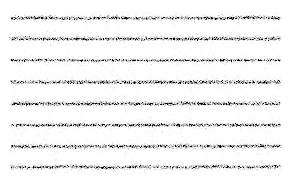
\includegraphics[width=\figone]{figs/fig_qc_linearity.pdf}
\caption{\label{fig:qc_linearity} \emph{Image of a line phantom acquired on a
gamma camera with poor linearity correction.}}
\end{figure}

\subsubsection{Dead time}
%--------------
The dead time measurements are based on some dead time model, for example
equations (\pref{eq:dead1}) or (\ref{eq:dead2}). The effective dead time $\tau$
is the parameter we want to obtain. Usually, the exact amount of radioactivity
is unknown as well, so there are two unknown variables. Consequently, we need
at least two measurements to determine them. Many procedures can be devised. A
straightforward one is to use a strong source with short half life, and
acquire images while the activity decays. At low count rates the gamma camera
is known to work well, so we assume that this part of the curve is correct
(slope 1). Thus, we can compute what the camera should have measured, the true
count rate, allowing us to draw the curve of figure \pref{fig:dead_time}. Then,
$\tau$ can be computed, e.g. by fitting the model to the rest of the curve.

A faster method suggested in \cite{Aanbevelingen} is to prepare two sources
with the same amount of radioactivity (difference less than 10\%). Select the
sources such that when combined the count rate is probably high enough to
produce a noticeable dead time effect (otherwise the subsequent analysis will
be very sensitive to noise). Put one source on the camera and measure the
count rate $R_1$. Put the second source on the camera and measure $R_{12}$.
Remove the first source and measure $R_2$. This produces the following
equations:
\begin{eqnarray}
    R_1    & = & R^\ast_1 e^{-R^\ast_1 \tau}\\
    R_2    & = & R^\ast_2 e^{-R^\ast_2 \tau}\\
    R_{12} & = & (R^\ast_1 + R^\ast_2) e^{-(R^\ast_1 + R^\ast_2) \tau},
\end{eqnarray}
where the (unknown) true count rates are marked with an asterisk. If we did a
good job preparing the sources, then we have $R_1 \simeq R_2$, so we can
simplify the equations into
\begin{eqnarray}
  R       & = & R^\ast e^{- R^\ast \tau}\\
  R_{12}  & = & 2 R^\ast e^{- 2 R^\ast \tau},
\end{eqnarray}
where we define $R = (R_1 + R_2) / 2$. A bit of work (left as an exercise
to the reader) leads to
\begin{equation}
  \tau = \frac{2 R_{12}}{(R_1 + R_2)^2} \ln \frac{R_1 + R_2}{R_{12}}.
\end{equation}

Knowing $\tau$, we can predict the dead time for any count rate, except for
very high ones (which should be avoided at all times anyway, because
in such a situation limited information is obtained at the cost of
increased radiation to the patient).

\subsubsection{Sensitivity}
%--------------
Sensitivity is measured by recording the count rate for a known radioactive
source. Because the measurement should not be affected by attenuation, NEMA
prescribes to use a recipient with a large (10 cm) flat bottom, with a bit of
water (3 mm high) to which about 10 MBq radioactive tracer has been added. The
result depends mainly on the collimator, and will be worse if the resolution
is better.

\subsection{Whole body imaging}
%==========================
A camera which is not ready for planar imaging, is obviously not ready
for whole body imaging either. In contrast, a camera that meets all
quality control criteria for planar imaging could still fail for whole
body imaging. There is only one essential difference between planar
imaging and whole body imaging: in whole body imaging the patient is
continuously moving with respect to the camera. In some systems the
patient bed is translated, in other systems the camera is moved, but
the potential problems are the same. During whole body imaging a
single large planar image is acquired (see figure
\pref{fig:planarwb}), which is as wide as the crystal (let us call
that the $x$-axis) but much longer (the $y$-axis). Consequently, the
coordinates $(x_{\mbox{wb}}, y_{\mbox{wb}})$ in the large image are
computed as
\begin{eqnarray}
  x_{\mbox{wb}} & = & x\\
  y_{\mbox{wb}} & = & y + v t,
\end{eqnarray}
where $(x,y)$ is the normal planar coordinate, $v$ is the table speed and $t$
is the time. The speed $v$ must be expressed in pixels per s, while the motor
of the bed is trying to move the bed at a predefined speed in cm per
s. Consequently, whole body image quality will only be optimal if
\begin{itemize}
  \item planar image quality is optimal, and
  \item the $y$-pixel size is exact, and
  \item the motor is working at the correct speed.
\end{itemize}

\subsubsection{Bed motion}
%--------------
The bed motion can be measured directly to check if the true scanning
speed is identical to the specified one.

\subsubsection{Uniformity}
%--------------
If the table motion is not constant, the image of a uniform source will not be
uniform. Of course, this uniformity test will also be affected if something is
wrong with planar performance. Uniformity is not affected if the motion is
wrong but constant, except possibly at the beginning and the end, depending on
implementation details.

\subsubsection{Pixel size, resolution}
%--------------
If there is something wrong with the conversion of table position to pixel
coordinate, this is very likely to affect the pixel size and spatial
resolution in the direction of table motion $y$. One can measure the pixel
size directly by measuring two points with very different
$y_{\mbox{wb}}$-coordinate. It is probably easier is to acquire a bar phantom
or line phantom, which gives an immediate impression of the spatial
resolution.


\subsection{SPECT}
%=================
A gamma camera which survives all quality control tests for planar
imaging may still fail for SPECT, since SPECT poses additional
requirements on the geometry of the system.

\subsubsection{Center-of-rotation}
%--------------
In SPECT, the gamma camera is used to acquire a set of sinograms, one for each
slice. Sinogram data are two-dimensional, one coordinate is the angle, the
other one the distance between the origin and the projection
line. Consequently, a sinogram can only be correctly interpreted if we know
which column in the image represents the projection line at zero distance. By
definition, this is the point where the origin, the rotation center is
projected.

\begin{figure}[t]
\centering
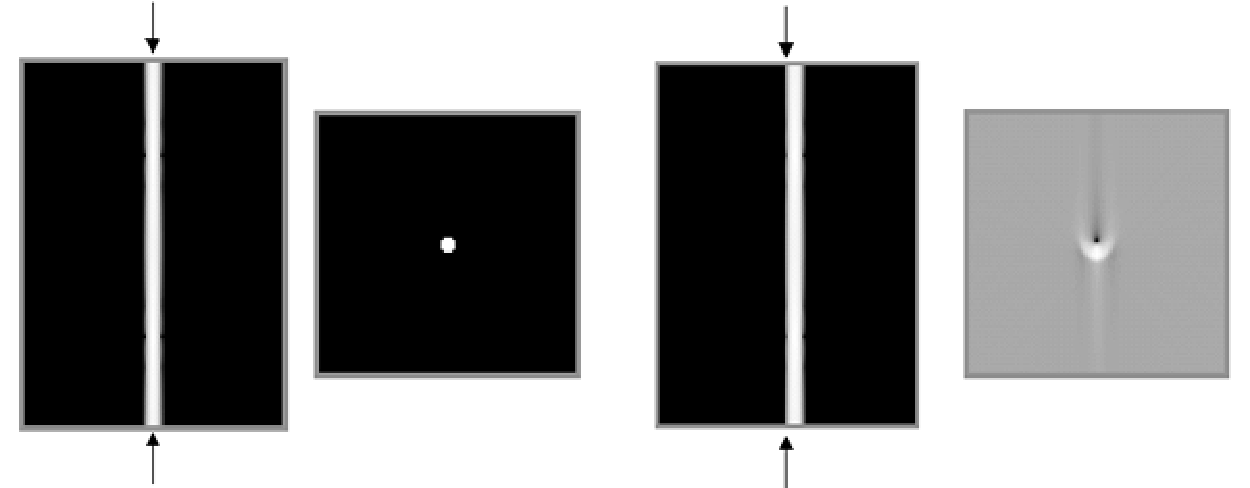
\includegraphics[width=\figbig]{figs/fig_cor.pdf}
\caption{\label{fig:cor} \emph{Simulation of center of rotation error. Left:
sinogram and reconstruction in absence of center of rotation error. Right:
filtered backprojection with center of rotation error equal to the diameter of
the point.}}
\end{figure}
%
For reasons of symmetry it is preferred (but not necessary) that the
projection of the origin is the central column of the sinogram, and
manufacturers attempt to obtain this. However, because of drift in the
electronics, there can be a small offset. This is illustrated in figure
\ref{fig:cor}. The leftmost images represent the sinogram of a point source
and the corresponding reconstruction if everything works well. The rightmost
images show what happens if there is a small offset between the projection of
the origin and the center of the sinogram (the position where the origin is
assumed to be during reconstruction, indicated with the arrows in the
sinogram). For a point source in the center, the sinogram becomes
inconsistent: the point is always at the right, no matter the viewing
angle. As a result, artifacts result in filtered backprojection (the
backprojection lines do not intersect where they should), which become more
severe with increasing center-of-rotation error.

From the sinogram, one can easily compute the offset. This is done by
fitting a sine to the mass center in each row of the sinogram,
determining the values of $A$, $\varphi$ and $B$ by minimizing
\begin{equation}
 \mbox{cost} = 
  \sum_i \left(m(\theta_i) 
           - (A \sin(\Delta_\theta \theta_i + \varphi) + B)\right)^2.
\end{equation}
The mass center, computed for each row $\theta_i$, represents the
detector position of the point source for the projection acquired at
angle $\Delta_\theta \theta_i$, where $\Delta_\theta \in \mathbb{R}$ is the
angle between subsequent sinogram rows, and $\theta_i \in \mathbb{N}$ is the
row index. The offset is the fitted value for $B$, while $A$ and
$\varphi$ are nuisance variables to be determined because we don't
know exactly where the point source was positioned. Once the offset is
known, we can correct for it, either by shifting the sinogram over $-B$,
or by telling the reconstruction algorithm where the true rotation
center is. SPECT systems software provides automated procedures which
compute the projection of the rotation axis from a point source
measurement. Older cameras suffered a lot from this problem, newer
cameras seem to be far more stable.


\subsubsection{Detector parallel to rotation axis}
%--------------
If the detector is not parallel to the rotation axis, the projections
for different angles are not parallel. This gives rise to serious
artifacts. Figure \ref{fig:gamma_parallel} shows that the projection
of a point source seems to oscillate parallel to the rotation axis
while the camera rotates (except for points on the rotation axis).

The figure tells the way to detect the error: put a point source in the field
of view, acquire a SPECT study and check if the point moves up and down in the
projections (or disappears from one sinogram to show up in the next one). For
a fixed angle, the amplitude of the apparent motion is proportional to the
distance between the point and the rotation axis. Nicely centered point
sources will detect nothing.

\begin{figure}[tb]
\centering
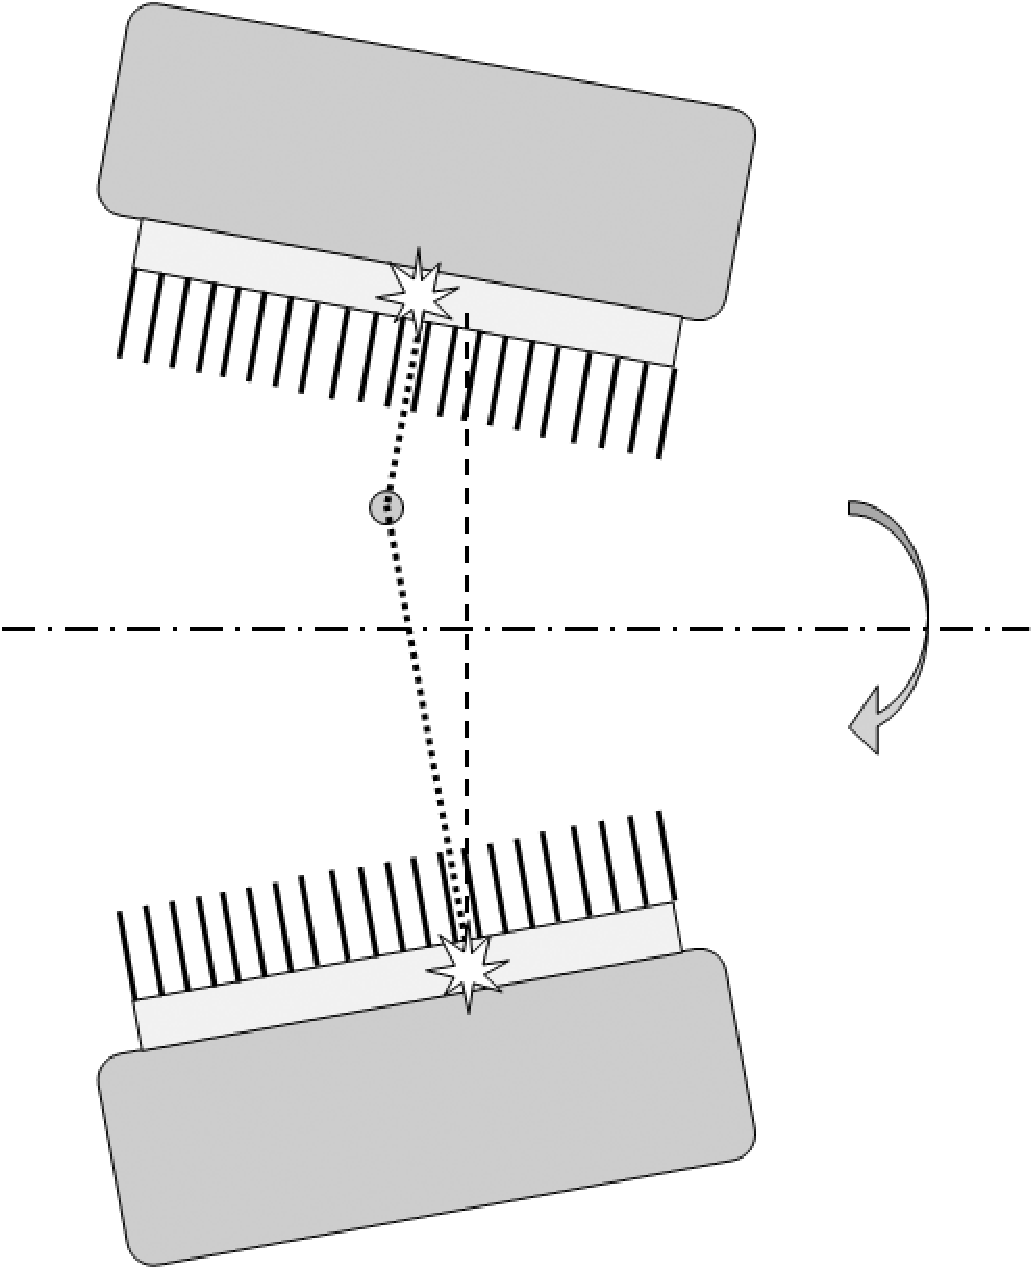
\includegraphics[width=0.7\figone]{figs/fig_gamma_parallel.pdf}
\caption{\label{fig:gamma_parallel} \emph{If the gamma camera is not parallel
to the rotation axis, a point apparently moves up and down the axis during
rotation.}}
\end{figure}


\subsubsection{SPECT phantom}
%--------------
It is a good idea to scan a complex phantom every now and then, and
compare the reconstruction to images obtained when the camera was
known to be tuned optimally. Several companies offer
polymethylmetacrylate (= perspex, Plexiglas) phantoms for this
purpose. The typical phantom is a hollow cylinder which must be filled
with water containing a radioactive tracer (fig
\ref{fig:jaszczak}). Various inserts are provided, e.g. sets of bars
of different diameter, allowing to evaluate the spatial resolution. A
portion of the cylinder is left free of inserts, allowing to check if
a homogeneous volume is reconstructed into a homogeneous image. Almost
any camera problem will lead to loss of resolution or loss of
contrast.

When filling a phantom with ``hot'' water, do not count on diffusion of the
tracer molecules to obtain a uniform distribution: it takes for ever before the
phantom is truly uniform. The water must be stirred.
\begin{figure}[tb]
\centering
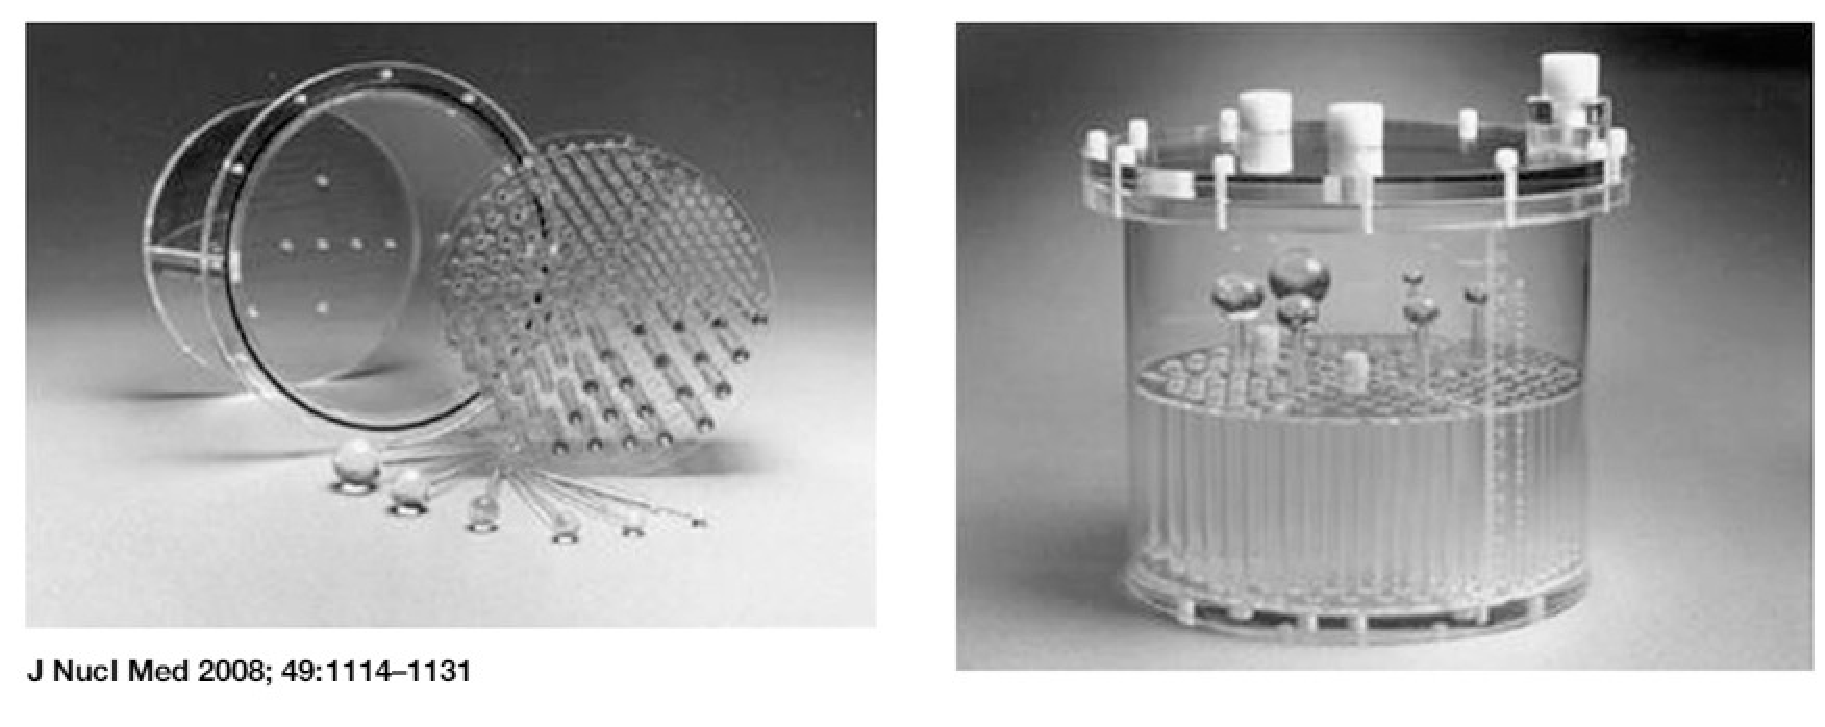
\includegraphics[width=1\figmedium]{figs/fig_jaszczakphantom.pdf}
\caption{\label{fig:jaszczak} \emph{A typical ``Jaszczak phantom'',
    named after a very well known SPECT researcher who developed many
    such phantoms (figure from P. Zanzonico, {\em J Nucl Med} 2008;
    49:1114-1131).}}
\end{figure}

\subsubsection{Quantification \label{sec:spectquant}}
%-----------------------------
In principle, a SPECT system can produce quantitative images, just
like a PET system, albeit with poorer resolution. This has long been
ignored in clinical practice, because absolute quantification usually
adds little diagnostic value. However, SPECT is increasingly being
used to prepare or verify radionuclide therapy treatments. In
radionuclide therapy, a large amount of a tumor-targetting
radiopharmacon is administered to the patient. The radiopharmacon
typically carries a beta- or alpha-emitter. In contrast to gamma
photons, these particles deposit their energy at short distances, and
when accumulated in the tumor lesions, they will deposit a large
amount of energy in the tumors and much less in the surrounding
healthy tissues. For those applications, it is important to determine
the exact amount of radioactivity in the tumors and healthy tissues,
to ensure that the tumors are destroyed and the damage to the healthy
tissues is as low as possible.

If the gamma camera is in good shape, and if the SPECT images are
reconstructed with attenuation correction and scatter correction, then
the reconstructed image pixel values should be proportional to the
local activity at that location. The constant of proportionality can
be obtained from a phantom measurement. A cylinder is filled with
water containing a well known uniform tracer concentration. The
cylinder is scanned and an image is reconstructed with attenuation and
scatter correction. Then the calibration factor is computed as the
ratio of the true tracer concentration in Bq/ml to the reconstructed
value. The reconstructed value is typically computed as the mean value
in a volume centered inside the phantom (this volume should stay away
from the phantom boundary, to avoid the influence of partial volume
effects). Multiplication of the reconstructed images with this
calibration factor converts them into quantitative images, with pixel
values giving the local activity in Bq/ml.

The calibration factor is tracer dependent, because the sensitivity of
the gamma camera to the radionuclide activity depends on the branching
ratio, on the energy (or energies) of the emitted photons and on the
collimator.

For ``well-behaved'' tracers which emit photons at a single energy
that is not too high, such as \textsuperscript{99m}Tc, the attenuation and scatter
correction is accurate. As a result, the calibration can be accurate
too. For tracers that emit photons at different energies, such as
$^{111}$In, attenuation and scatter correction is more
difficult. Scatter correction is more complicated because the Compton
scattered photons from the high energy peak may end up in the low
energy window. Attenuation correction is more complicated because the
attenuation is energy dependent. For such tracers, accurate
quantification is still possible, but it is more challenging.

The calibration factor must be verified, and corrected if necessary, a
few times per year, to ensure that the SPECT system remains
quantitatively accurate.

\section{Positron emission tomograph}
%%%%%%%%%%%%%%%%%%
A PET-system is more expensive and more complicated than a gamma camera,
because it contains more and faster electronics. However, in principle,
it is easier to tune. The reason is that a multicrystal design has some
robustness because of its modularity: if all modules work well, the whole
system works well. A module contains only a few PMT's and a few crystals, and
keeping such a small system well-tuned is ``easier'' than doing the same for a
large single crystal detector.

\subsection{Evolution of blank scan}
%==========
Older PET-systems have computer controlled transmission sources: the
computer can bring them in the field of view, and can have them
retracted into a shielding container. When the transmission rod
sources are extended they are continuously rotated near the perimeter
of the field of view, such that all projection lines will be
intersected.

A new blank scan is automatically acquired in the early morning,
before working hours. This blank scan is a useful tool for performance
monitoring, since all possible detector pairs contribute to it.  The
daily blank scan is compared to the reference blank scan, and
significant deviations are automatically detected and reported, so
drift in the characteristics is soon detected. If a problem is found
it must be remedied. Often it is sufficient to redo calibration and
normalization (see below). Possibly a PMT or an electronic module is
replaced, followed by calibration and normalization. When the system
is back in optimal condition, a new reference blank scan is acquired.

With the introduction of PET/CT, PET-systems no longer have these
built-in transmission sources. Therefore, the procedure has been
adapted such that it works with smaller phantoms, e.g. a cylinder
(typically with diameter of about 20 cm) filled with a solid solution
containing $^{68}$Ge. All detectors still cotnribute to the scan of
such a phantom, but there are now many detector {\em pairs} that will
see no counts, because they don't intersect the phantom. Therefore,
the performance of these detector pairs must be deduced from the
performance of the individual detectors.


\subsection{Normalization}
%==========
Normalization is used to correct for non-uniformities in PET detector
sensitivities (see section \pref{sec:normalization1}). The
manufacturers provide software to compute and apply the sensitivity
correction based on a scan of a particular phantom (e.g. a radioactive
cylinder positioned in the center of the field of view). Current
PET/CT (or PET/MR) systems do not have a transmission scan. Instead of
the blank scan, they use a scan of this phantom to detect, quantify
and correct changes in detector performance over time.

\subsection{Front end calibration}
%==========
The term ``calibration'' refers here to a complex automated procedure
which
\begin{itemize}
  \item tunes the PMT-gains to make their characteristics as similar as
        possible,
  \item determines the energy and position correction matrices for each
        detector module,
  \item determines differences in response time (a wire of 1 m adds 3
        ns under optimal conditions) and uses that information to make
        the appropriate corrections, to ensure that the coincidence
        window (about 10 ns in non-TOF PET and around 500 ps in
        TOF-PET) meets its specifications.
\end{itemize}
The first two operations are performed with a calibrated phantom carefully
positioned in the field of view, since 511 keV photons are needed to measure
spectra and construct histograms as a function of position. The timing
calibration is based on purely electronic procedures, without the phantom
(since one cannot predict when the photons will arrive).

\subsection{Quantification \label{sec:scalefactor}}
%==========
When a PET system is well tuned, the reconstructed intensity values
are proportional to the activity that was in the field of view during
the PET scan. This constant of proportionality (called {\em
calibration factor} or {\em PET scale factor} or so) is determined
from a phantom measurement. A cylinder is filled with a well known and
uniform tracer concentration, and a PET scan is acquired. The
calibration factor is computed as the ratio of the reconstructed value
to the true tracer concentration in Bq/ml.  The reconstructed value is
typically computed as the mean value in a volume centered inside the
phantom (this volume should stay away from the phantom boundary, to
avoid the influence of partial volume effects). Once the system knows
this ratio, its reconstruction program(s) produce quantitative images
of the measured tracer concentration in Bq/ml. The calibration factor
must be verified, and corrected if necessary, a few times per year, to
ensure that the PET system remains quantitatively accurate.